%============================================================================%
%
%	DOCUMENT DEFINITION
%
%============================================================================%


% Using article class because we want to fully customize the page and don't use a cv template
\documentclass[10pt, letter]{article}	


%----------------------------------------------------------------------------------------
% Colors
%---------------------------------------------------------------------------------------- 
\usepackage{transparent}
\usepackage{xcolor}

% primary color
\definecolor{maincol}{RGB}{ 255, 0, 0 }

% dark color
\definecolor{darkcol}{RGB}{ 70, 70, 70 }

% light color
\definecolor{lightcol}{RGB}{245,245,245}

%----------------------------------------------------------------------------------------
%	ENCODING
%----------------------------------------------------------------------------------------

% we use utf8 since we want to build from any machine
\usepackage[utf8]{inputenc}		

%----------------------------------------------------------------------------------------
%	LOGIC
%----------------------------------------------------------------------------------------

% provides \isempty test
\usepackage{xstring, xifthen}

%----------------------------------------------------------------------------------------
%	FONT BASICS
%----------------------------------------------------------------------------------------

% some tex-live fonts - choose your own

%\usepackage[defaultsans]{droidsans}
%\usepackage[default]{comfortaa}
%\usepackage{cmbright}
\usepackage[default]{raleway}
%\usepackage{fetamont}
%\usepackage[default]{gillius}
%\usepackage[light,math]{iwona}
%\usepackage[thin]{roboto} 

% set font default
\renewcommand*\familydefault{\sfdefault} 	
\usepackage[T1]{fontenc}

% more font size definitions
\usepackage{moresize}

%----------------------------------------------------------------------------------------
%	FONT AWESOME ICONS
%---------------------------------------------------------------------------------------- 

% include the fontawesome icon set
\usepackage{fontawesome}

% use to vertically center content
% credits to: http://tex.stackexchange.com/questions/7219/how-to-vertically-center-two-images-next-to-each-other
\newcommand*{\vcenteredhbox}[1]{
    \begingroup
        \setbox0=\hbox{#1}\parbox{\wd0}{\box0}
    \endgroup
}

% icon shortcut
\newcommand{\icon}[3] { 	
    \makebox(#2, #2){\color{maincol}{\csname fa#1\endcsname}}
}	

% icon with text shortcut
\newcommand{\icontext}[4]{ 		
    \vcenteredhbox{\icon{#1}{#2}{#3}}
    \hspace{2pt}
    \parbox{\mpwidth}
    {\color{#4}{#3}}
}


% icon with website url
\newcommand{\iconhref}[5]{ 						
    \vcenteredhbox{\icon{#1}{#2}{#5}}
    \hspace{2pt} 
    \href{#4}{\color{#5}{#3}}
}

% icon with email link
\newcommand{\iconemail}[5]{ 						
    \vcenteredhbox{\icon{#1}{#2}{#5}}
    \hspace{2pt}
    \href{mailto:#4}{\color{#5}{#3}}
}

%----------------------------------------------------------------------------------------
%	PAGE LAYOUT  DEFINITIONS
%----------------------------------------------------------------------------------------

% page outer frames (debug-only)
%\usepackage{showframe}		

% we use paracol to display breakable two columns
\usepackage{paracol}

% define page styles using geometry
\usepackage[letter]{geometry}

% remove all possible margins
\geometry{top=0.5in, bottom=0.5in, left=0.5in, right=0.5in}

\usepackage{fancyhdr}
\pagestyle{empty}


% indentation is zero
\setlength{\parindent}{0in}

%----------------------------------------------------------------------------------------
%	TABLE /ARRAY DEFINITIONS
%---------------------------------------------------------------------------------------- 

% extended aligning of tabular cells
\usepackage{array}

% custom column right-align with fixed width
% use like p{size} but via x{size}
\newcolumntype{x}[1]{%
>{\raggedleft\hspace{0pt}}p{#1}}%


%----------------------------------------------------------------------------------------
%	GRAPHICS DEFINITIONS
%---------------------------------------------------------------------------------------- 

%for header image
\usepackage{graphicx}


%for drawing graphics		
\usepackage{tikz}				
\usetikzlibrary{shapes, backgrounds, mindmap, trees}


% Package for links, must be the last package used
\usepackage[hidelinks]{hyperref}

% returns minipage width minus two times \fboxsep
% to keep padding included in width calculations
% can also be used for other boxes / environments
\newcommand{\mpwidth}{\linewidth-\fboxsep-\fboxsep}


%============================================================================%
%
%	CV COMMANDS
%
%============================================================================%

%----------------------------------------------------------------------------------------
%	 CV LIST
%----------------------------------------------------------------------------------------

% renders a standard latex list but abstracts away the environment definition (begin/end)
\newcommand{\cvlist}[1] {
    \begin{itemize}
        \itemsep 0em 
        {#1}
    \end{itemize}
}

%----------------------------------------------------------------------------------------
%	 CV TEXT
%----------------------------------------------------------------------------------------

% base class to wrap any text based stuff here. Renders like a paragraph.
% Allows complex commands to be passed, too.
% param 1: *any
\newcommand{\cvtext}[1] {
    \setlength{\tabcolsep}{0pt}
    \begin{tabular*}{\mpwidth}{p{1.03\mpwidth}}
        \parbox{\mpwidth}{#1}
    \end{tabular*}
}

%----------------------------------------------------------------------------------------
%	CV SECTION
%----------------------------------------------------------------------------------------

% Renders a a CV section headline with a nice underline in main color.
% param 1: section title
\newcommand{\cvsection}[1] {
    \vspace{6pt}
    \cvtext{
        \textbf{\LARGE{\color{darkcol}{\uppercase{#1}}}}\\[-6pt]
        \color{maincol}{ \rule{0.1\textwidth}{1pt} } \\
    }
}

%----------------------------------------------------------------------------------------
% Skill
%----------------------------------------------------------------------------------------

% Renders a progress-bar to indicate a certain skill in percent.
% param 1: name of the skill / tech / etc.
% param 2: level (for example in years)
% param 3: percent, values range from 0 to 1
\newcommand{\cvskill}[3] {
    \setlength{\tabcolsep}{0pt}
    \begin{tabular*}{1\mpwidth}{@{\extracolsep{\fill}} l r}
        \color{black}{\textbf{#1}} & \color{maincol}{#2}\\
    \end{tabular*}%
}


%----------------------------------------------------------------------------------------
%	 CV EVENT
%----------------------------------------------------------------------------------------

% Renders a table and a paragraph (cvtext) wrapped in a parbox (to ensure minimum content
% is glued together when a pagebreak appears).
% Additional Information can be passed in text or list form (or other environments).
% the work you did
% param 1: Timeframe i.e. Sep 14 - Jan 15 or 2015 - 2018
% param 2: Event (Title, Job Position, etc.)
% param 3: Customer, Employer, Industry
% param 4: Short description
% param 5: Work (optional)
% param 6: Technologies include (optional)
% param 7: Achievements (optional)
\newcommand{\cvevent}[7] {
	
    % we wrap this part in a parbox, so title and description are not separated on a pagebreak
    % if you need more control on page breaks, remove the parbox
    \parbox{\mpwidth}{
        \setlength{\tabcolsep}{0pt}
        \begin{tabular*}{1.035\mpwidth}{@{\extracolsep{\fill}} l r}
            \color{black}{\large{\textbf{#2}}}        & 
            \colorbox{maincol}{
                \makebox[0.32\mpwidth]{
                    \color{white}\large{{#1}}
                }
            } \\
            \color{maincol}{\large{\textbf{#3}}}  &  \\
        \end{tabular}
        \vspace{6pt}
        
        \ifthenelse{\isempty{#4}}{}{
            \cvtext{#4}\\
        }
    }
    
    \ifthenelse{\isempty{#5}}{}{
        {#5}
    }
    
    \ifthenelse{\isempty{#6}}{}{
        \cvtext{\textbf{Technologies:}}
        {#6}
    }
    
    \ifthenelse{\isempty{#7}}{}{
        \cvtext{\textbf{Achievements:}}
        {#7}
    }
    \vspace{6pt}
}

%----------------------------------------------------------------------------------------
% CV Meta Event
%----------------------------------------------------------------------------------------

% Renders a CV event on the sidebar
% param 1: title
% param 2: subtitle (optional)
% param 3: customer, employer, etc,. (optional)
% param 4: info text (optional)
\newcommand{\cvmetaevent}[4] {
    \color{maincol}{\cvtext{\textbf{#1}}}
    
    \ifthenelse{\isempty{#2}}{}{
    \color{darkcol}{\cvtext{\textbf{#2}} }
    }
    
    \ifthenelse{\isempty{#3}}{}{
        \cvtext{{ \color{darkcol} {#3} }}\\
    }
    
    \color{black}\cvtext{#4}\\
    [10pt]
}

%----------------------------------------------------------------------------------------
%	 CV Patent Event
%----------------------------------------------------------------------------------------

% Renders a CV Patent event on the sidebar
% param 1: title
% param 2: Year
% param 3: Link
% param 4: Info text (optional)
\newcommand{\cvpatentevent}[4] {
    \color{maincol}{\cvtext{\textbf{#1}}}


    \begin{tabular*}{1.035\mpwidth}{@{\extracolsep{\fill}} l r}
        \color{black}{\large{\textbf{#2}}}        & 
        \iconhref{Link}{6}{Link}{#3}{black} \\
    \end{tabular}\\

    \color{black}\cvtext{#4}\\[12pt]
}

%---------------------------------------------------------------------------------------
%	QR CODE
%---------------------------------------------------------------------------------------

% Renders a qrcode image (centered, relative to the parentwidth)
% param 1: percent width, from 0 to 1
\newcommand{\cvqrcode}[1] {
    
\includegraphics[width={#1}\linewidth]{images/qrcode.png}
}


%============================================================================%
%
%
%
%	DOCUMENT CONTENT
%
%
%
%============================================================================%
\begin{document}

%---------------------------------------------------------------------------------------
% Setup Metadata for PDF Compilation
%----------------------------------------------------------------------------------------
%---------------------------------------------------------------------------------------
% Setup Metadata for PDF Compilation
%----------------------------------------------------------------------------------------
\hypersetup{pdfauthor={Richard Hoehn},%
            pdftitle={Resume of Richard Hoehn},%
            pdfsubject={This PDF is the resume of Richard Hoehn. This resume was compiled by Richard Hoehn on \today} via the LaTex application he wrote in May of 2024. Copyright © 2024 Richard Hoehn,%
            pdfkeywords={Resume, AWS, Computer Engineering, Computer Science, PostgreSQL, International Travel, MBA, PhD, MS, BS, Nasville, Tennessee, Management, Founder, Co-Founder, Execution, Software Architecture, Node.JS, Vue.JS, Flutter, Dart, JavaScript, RESTful, API, SQS, SNS, SMTP, Database, Hadoop, Spark, Machine Learning, Deep Learing, AI, },%
            pdfproducer={LaTeX},%
            pdfcreator={Richard Hoehn}
}


\columnratio{0.35}
\setlength{\columnsep}{1em}
\setlength{\columnseprule}{1pt}
\colseprulecolor{lightcol}

\begin{paracol}{2}
\begin{leftcolumn}
%---------------------------------------------------------------------------------------
% Profile Image
%----------------------------------------------------------------------------------------
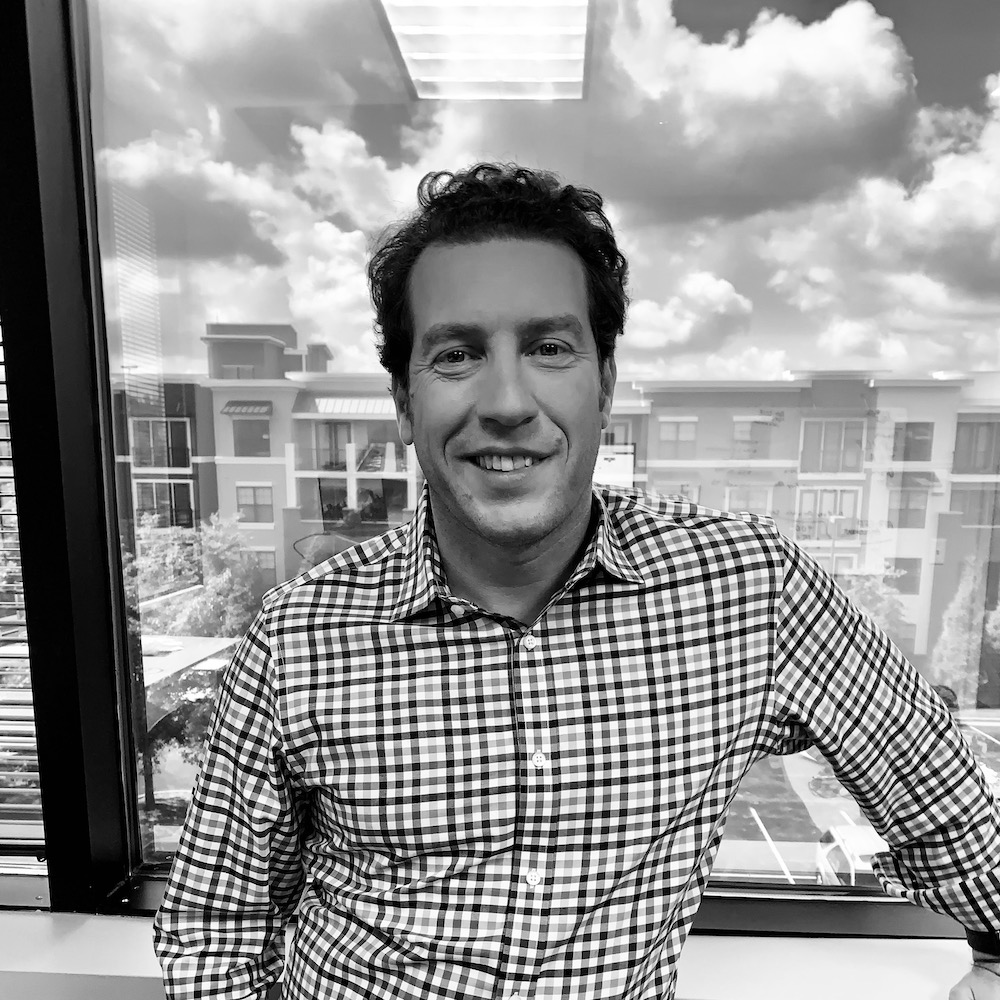
\includegraphics[width=\linewidth]{images/Richard-Head-Square-Small.jpeg}

%---------------------------------------------------------------------------------------
% Profile
%---------------------------------------------------------------------------------------
\vfill\null
%---------------------------------------------------------------------------------------
% Profile
%----------------------------------------------------------------------------------------
\cvsection{PROFILE}

\cvtext{
Dynamic and innovative professional with a talent for identifying and resolving complex issues. Known for optimizing business processes and swiftly addressing challenges with a hands-on approach.\\[6pt]
Currently leading a product development and consulting firm, leveraging industry experience and innovative thinking to deliver lasting solutions. Skilled in developing hardware and software products for diverse industries. Proven startup founder with a track record of building and selling companies. Committed to driving technological advancements and achieving business excellence.
}

%---------------------------------------------------------------------------------------
% Contact
%---------------------------------------------------------------------------------------
%---------------------------------------------------------------------------------------
% Contact
%---------------------------------------------------------------------------------------
\vfill\null
\vfill\null
\cvsection{CONTACT}
	
\icontext{MapMarker}{6}{Nashville, TN, USA}{black}\\[6pt]
\icontext{MobilePhone}{6}{+1 615 319-2171}{black}\\[6pt]
\iconemail{Envelope}{6}{rhoehn@gmail.com}{rhoehn@gmail.com}{black}\\[6pt]
\iconhref{Linkedin}{6}{LinkedIn}{https://linkedin.com/in/richardhoehn/}{black}\\[6pt]
\iconhref{Link}{6}{www.RichardHoehn.com}{https://richardhoehn.com/}{black}\\[6pt]


%---------------------------------------------------------------------------------------
% QR Code
%--------------------------------------------------------------------------------------
\vfill\null
\cvqrcode{0.4}


\newpage


%---------------------------------------------------------------------------------------
% Education
%----------------------------------------------------------------------------------------
%---------------------------------------------------------------------------------------
% Education
%---------------------------------------------------------------------------------------
\newpage
\cvsection{EDUCATION}

\cvmetaevent
{2022 - Current}
{PhD Computational Data}
{Middle TN State Univ. (MTSU)}
{
Specializing in advanced algorithms, data analysis, and machine learning techniques to solve complex problems in diverse industries.\\

Developed and refined predictive models that improved decision-making processes, contributing to several papers on data optimization and efficiency in NLP, Finance, and HR Resume tracking.
}

\vfill\null
\cvmetaevent
{2007 - 2009}
{MBA Executive}
{Vanderbilt University}
{
Earned an Executive MBA from Vanderbilt University, gaining advanced management training and strategic decision-making skills that have been directly applied to current professional challenges.
}

\vfill\null
\cvmetaevent
{2022 - 2025}
{MS Data Science}
{Middle TN State Univ. (MTSU)}
{
A strong focus on predictive analytics, machine learning, and statistical modeling. Applied comprehensive knowledge to real-world data sets during projects, enhancing predictive accuracy and decision-making capabilities for business applications.
}

\vfill\null
\cvmetaevent
{2002 - 2006}
{BS Computer Engineering \& Science}
{Middle TN State Univ. (MTSU)}
{
B.S. in Computer Engineering and Computer Science from Middle Tennessee State University, graduated with a 3.9 GPA, mastering software development, system architecture, and hardware integration. Leveraged expertise in both engineering and programming to design and optimize innovative computing solutions and applications.
}


\newpage

%---------------------------------------------------------------------------------------
% Language
%----------------------------------------------------------------------------------------
%---------------------------------------------------------------------------------------
% Languages
%---------------------------------------------------------------------------------------

\cvsection{International}

\textcolor{maincol} {\cvtext{\textbf{\begin{flushleft}Languages\end{flushleft}}}}\\
\icontext{CommentO}{15}{English - Native / Bilingual}{black}\\
\icontext{CommentO}{15}{German - Native / Bilingual}{black}\\
\icontext{CommentO}{15}{French - Conversational}{black}\\

\textcolor{maincol} {\cvtext{\textbf{\begin{flushleft}Work Authorization\end{flushleft}}}}\\
\icontext{Globe}{15}{US Citizen}{black}\\
\icontext{Globe}{15}{Swiss Citizen}{black}\\
\icontext{Globe}{15}{Canadian Citizen}{black}\\


\vfill\null

%---------------------------------------------------------------------------------------
% Patents
%---------------------------------------------------------------------------------------
%---------------------------------------------------------------------------------------
% Patents
%---------------------------------------------------------------------------------------
\cvsection{Patents}


\cvpatentevent
{SECURITY TAG GROUPING}
{2016}
{https://patents.google.com/patent/US20160180672A1}
{A device control to interface with a plurality of security tags adapted to be disposed on a corresponding plurality of products in a monitoring environment.}


\cvpatentevent
{SECURITY TAG POSITIONING}
{2016}
{https://patents.google.com/patent/US9373237B1}
{A controller configured with a security tag adapted to be disposed on a corresponding product in a monitoring environment.}


\cvpatentevent
{SECURITY TAG ALERTING FOR CONTINUOUS MOVEMENT}
{2016}
{https://patents.google.com/patent/US20160180671A1}
{A method for interaction analysis, focusing on providing insights into behaviors and preferences based on interactions with electronic devices}


\cvpatentevent
{Stylus for use with touch screen computing device}
{2011}
{https://patents.google.com/patent/US20130050154A1}
{A pen or stylus for use with a touch screen computer (iPad).}


\cvpatentevent
{Inkjet cartridge refilling machine with improved refill process}
{2007}
{https://patents.google.com/patent/US20070285475A1}
{A method is provided for refilling an ink reservoir associated with an ink jet printer cartridge containing foam material in the cartridge.}



\end{leftcolumn}

\begin{rightcolumn}

%---------------------------------------------------------------------------------------
% Title Header Rectangle
%---------------------------------------------------------------------------------------
\fcolorbox{white}{darkcol}{\begin{minipage}[c][0.8in][c]{1\mpwidth}
    \begin {center}
        \HUGE{ \textbf{ \color{white}{ \uppercase{ Richard Hoehn } } } }\\[6pt]
        \large{ \color{white} {+20 yrs Development, Code, and Leadership Experience} }
    \end {center}
\end{minipage}}

\vfill\null


%---------------------------------------------------------------------------------------
% Introduction
%---------------------------------------------------------------------------------------
%---------------------------------------------------------------------------------------
% Intro
%----------------------------------------------------------------------------------------
\cvsection{Introduction}

\cvtext{
Seasoned business professional with a proven track record of launching and exiting successful startups, equipped with 20+ years of software, hardware, and consumer electronics development experience supported by an MBA and Computer Science degrees.\\
}

%---------------------------------------------------------------------------------------
% Experience
%---------------------------------------------------------------------------------------
%---------------------------------------------------------------------------------------
% Experience
%---------------------------------------------------------------------------------------
\vfill\null
\cvsection{WORK EXPERIENCE}

\cvevent
{2023 - Present}
{Hoehn Innovations, LLC.}
{Owner / Founder}
{At Hoehn Innovations, I work on finding innovative solutions using technology,
process design, and with those tools specializing in creating meaningful hard \& software products for various industries. My role is to contribute technical guidance by conceptualizing and developing innovative solutions to address complex challenges for our clients.}
% Simple Bullets
{\cvlist{
    \item Flutter \& Dart for Mobile Application Development
    \item Vue.JS, Node.JS, PostgreSQL, AWS Full Suite, GCP Firebase
    \item PyTorch \& Torch Lighting Module Design
}}
% Technologies
{} % None
% Achievements
{\cvlist{
    \item Launched Bluetooth device on Amazon with +250 units a month sold
    \item Deployed ML resume scan app to predict employee Turn-over
    \item Tools for RESTful API integration using Pub Sub technologies on AWS
}}


\vfill\null
\cvevent
{2015 - 2022}
{FreightWise, LLC.}
{CTO / CIO / Co-Founder}
{Co-Founded and exited a successful Logistics Technology company providing TMS SaaS \& Managed Transportation services. FreightWise technology optimizes freight profiles and streamlines TMS \& WMS operations.\\[6pt]
In 2019 FreightWise was the 2\textsuperscript{nd} fastest growing company in the US, and the fastest growing company in Nashville four years in a row, 2019-2023.\\[6pt]
Technologies such as Node.JS, PostgreSQL, Docker, AWS, and event-driven programming by use of Kafka delivering real-time web, mobile, and desktop apps.}
{\cvlist{
    \item CTO - Wrote the first lines of code - Exited with 20 developers on staff
    \item Managed Product Mgmt. Team - Applied Pragmatic Marketing principles
    \item Created Customer Solutions Team as an integrated service center withing our SaaS application
    \item Initiated and helped bring to market Cargo Insurance offering within the SaaS platform
}}
{}
{}


\vfill\null
\cvevent
{2015 - 2018}
{Canary Computer Engineering}
{CEO / Co-Founder}
{Architected, designed (hardware \& software), and deployed +300 units at multiple large retailers an event-driven IoT (Internet of Things) platform.\\[6pt]
We used LTE CAT-M1 networks to ensure our devices are the most energy efficient on the market. By integrating a dedicated SSH tunnel between the devices and AWS SQS platform.}
{\cvlist{
    \item Networks using Bluetooth 4.2 \& 5.0 for large range internal applications and LTE CAT-M1 for energy efficient distributed networks.
    \item Develops iOS and Android apps using React Native, ES2015, JAVA, Objective-C, and Swift
}}
{}
{}


\vfill\null
\cvevent
{2012 - 2015}
{Checkpoint Systems}
{Dir. Global Product Management}
{Checkpoint Systems is a global leader in technology solutions for retail, including RFID, EAS (Electronic Article Surveillance), and loss prevention, aimed at improving inventory accuracy and operational efficiency.\\[6pt]I was tasked with completing and deploying a \$2M product to all of North America and Europe in high-end retail stores.}
{\cvlist{
    \item Developed and deployed a \$2M development project for in-store GPS
    \item Traveled extensively to introduce, train, and sell S3i product line I manged
    \item Managed with internal marketing team the successful launch of S3i to numerous USA, Canadian, France, and Netherlands retailers
}}
{}
{}


\vfill\null
\cvevent
{2010 - 2012}
{Griffin Technology}
{EE \& FW Manager}
{
Griffin Technology designed and manufactured technical solutions with an innovative flair. They grew during to become one of the largest providers of accessories for iPhone and Android media. Some of the best known accessories I worked on included the iTrip family of FM transmitters and the groundbreaking Evolve Wireless Sound System.\\[6pt]I managed the electrical and firmware engineering group of 10 members and interacted extensively with the our counterparts in Asia.
}
{\cvlist{
    \item Managed 4 embedded software and firmware developers
    \item Managed 5 electrical and PCB layout engineers
    \item Managed the E-Emissions and Prototype assembly lab and respective technicians
    \item Personally contributed firmware for embedded devices: Bluetooth, TCP/IP, IoT and IR devices
    \item Worked heavily in MySQL and SQL-Server backend IoT applications
}}
{}
{}


\vfill\null
\cvevent
{2007 - 2010}
{Big Time Toys, LLC.}
{Dir. of Manufacturing}
{I spent close to 120 days of the year in Asia. I flew back and forth between Asia on a 4-6week basis. This ensured the cultivation of strong relationships with our Asian partners and local development and management team, which enabled the lowering of cost, payment terms, and bringing products faster and more efficiently to market.}
{\cvlist{
    \item Extensive travel to China, Vietnam, and Europe
    \item Developed, priced, and delivered primarily electronics toys in the USA, HKG, and China
    \item Worked on establishing manufacturing options in Vietnam as supply chain risk management strategy 
    \item Worked with Walmart, Target, Toys Are Us, Costco, and numerous European \& Australian retail distribution  
    \item I spent close to 120 days of the year in Asia
}}
{}
{}

\vfill\null

%---------------------------------------------------------------------------------------
% Skills
%---------------------------------------------------------------------------------------
%---------------------------------------------------------------------------------------
% Skills
%----------------------------------------------------------------------------------------
\cvsection{Skills}

\textcolor{maincol} {\cvtext{\textbf{\begin{flushleft}Managerial\end{flushleft}}}}\\
\cvlist{
    \item \cvskill{Founder, CTO, \& Exit Experience to Private Equity (PE)} {5+ yrs}\\
    \item \cvskill{Team Building \& Product Management \& Product Delivery} {15+ yrs}\\
    \item \cvskill{Product Development, MVP Creation, Deployments} {10+ yrs}\\
    \item \cvskill{Extensive ravel: US, China, HKG, Europe, \& Australia} {15+ yrs}\\
    \item \cvskill{Business Finance, Valuation of Tech, Exit Valuations} {5+ yrs}\\
    \item \cvskill{Debt. Acquisition, Debt. Covenants, and Revenue Mgmt.} {3+ yrs}\\
}


\textcolor{maincol} {\cvtext{\textbf{\begin{flushleft}Technical\end{flushleft}}}}\\
\cvlist{
    \item \cvskill{Python, Node.JS, C\#, Dart, Javascript, SQL} {20+ yrs}\\
    \item \cvskill{Vue.JS, Angular, Flutter, React} {10+ yrs}\\
    \item \cvskill{PostgreSQL, Mongo, MS-SQL, MySQL, MemCache, Redis} {15+ yrs}\\
    \item \cvskill{Elastic Search, AWS Cloud Search, Splunk} {5+ yrs}\\
    \item \cvskill{AWS, SQS, SNS, S3, CloudFormation, YAML, Lambdas} {10+ yrs}\\
    \item \cvskill{GCP, Firebase, Dart} {5+ yrs}\\
    \item \cvskill{Docker, Imaging, ECS, NGINX} {5+ yrs}\\
    \item \cvskill{RESTful, API, Postman, Mocha, Puppeteer} {5+ yrs}\\
    \item \cvskill{GIT, CodePush, General Development Lifecycle, Agile} {10+ yrs}\\
}



\end{rightcolumn}
\end{paracol}
\end{document}

